
%%%%%%%%%%%%%%%%%%%%%%%%%%%%%%%%%%%%%%%%%%%%%%%%%%%%%%%%%%%%%%%%%%%%%%%%%%

\section*{Problema \textcolor{CIMATRed}{1}}

Se tiene la siguiente tabla donde se eligen varios niveles de ronquidos y se ponen en relación con una enfermedad cardíaca. Se toman como puntuaciones relativas de ronquidos los valores $\{0, 2, 4, 5\}$.

\begin{center}
\begin{tabular}{lccc}
\toprule
& \multicolumn{2}{c}{\textbf{Enfermedad Cardíaca}} & \\
\cmidrule(lr){2-3}
\textbf{Ronquido} & \textbf{SI} & \textbf{NO} & \textbf{Proporción de SI} \\
\midrule
Nunca & 24 & 1355 & 0.017 \\
Ocasional & 35 & 603 & 0.055 \\
Casi cada noche & 21 & 192 & 0.099 \\
Cada noche & 30 & 224 & 0.118 \\
\bottomrule
\end{tabular}
\end{center}

Ajuste un modelo lineal generalizado \textbf{logit} y \textbf{probit} (\textbf{investigar sobre el link probit}) para analizar si existe una relación entre los ronquidos y la posibilidad de tener una enfermedad cardíaca.\\

\noindent\fbox{\textbf{SOLUCIÓN}}\\

\textit{Se utilizo el lenguaje de programación \texttt{R} para resolver este problema, el código utilizado se encuentran al final del documento en el apéndice} \textbf{A.1}

Primero recordemos que el propósito de una función de enlace en un GLM busca modelar la relación entre uno o más predictores $X$ y una variable de respuesta $Y$. La función de enlace $g$, es el puente que conecta el predictor lineal, $\eta = \beta_0 + \beta_1X_1 + \dots$, con el valor esperado de la variable de respuesta $\mu = E(Y)$. Su forma fundamental es: 
\begin{equation}
    g(\mu) = \eta    
\end{equation}

En este problema, la respuesta es binaria (Sí/No enfermedad), por lo que su valor esperado es una probabilidad, sea $\pi = P(Y=1)$, que siempre está entre 0 y 1. Sin embargo, el predictor lineal $\eta$ puede tomar cualquier valor real de $-\infty$ a $+\infty$. La función de enlace se encarga de mapear el rango $(0, 1)$ de la probabilidad al rango $(-\infty, +\infty)$ del predictor lineal. El \textbf{enlace logit}, utiliza la función logaritmo de las ``odds'' (razón de momios) que habíamos visto antes: 
\begin{equation}
    g(\pi) = \ln\left(\frac{\pi}{1-\pi}\right)
\end{equation}
   
Esta función es la inversa de la función de distribución acumulada, CDF, de la distribución logística estándar. Por otra parte el \textbf{enlace probit} es muy similar conceptualmente, pero utiliza una distribución diferente como base, esta es la función cuantil:
\begin{equation}
    g(\pi) = \Phi^{-1}(\pi)
\end{equation}
    
Donde la funcion cuantil $\Phi^{-1}$ es la inversa de la CDF de la distribución normal estándar, $N(0, 1)$. En otras palabras, la función probit toma una probabilidad $\pi$ y te devuelve el puntaje Z (z-score) correspondiente a esa probabilidad.

Entonces, para resolver el problema primero cargamos los datos manualmente en un data frame y se procedió a ajustar los modelos logit y probit obteniendo los siguientes resultados respectivamente:

\begin{table}[H]
\centering
\caption{Resumen del ajuste del modelo Logit}
\label{tab:logit_summary}
\begin{tabular}{lrrrr}
\hline
 & \textbf{Estimate} & \textbf{Std. Error} & \textbf{z value} & \textbf{Pr($\mathbf{>|z|}$)} \\
\hline
\textbf{Intercept} & -3.86625 & 0.16621 & -23.261 & $<2 \times 10^{-16}$$^{***}$ \\
\textbf{score}     & 0.39734  & 0.05001 & 7.945   & $1.94 \times 10^{-15}$$^{***}$ \\
\hline
\multicolumn{5}{l}{\footnotesize Signif. codes: $^{***}0.001$, $^{**}0.01$, $^{*}0.05$, $^{.}0.1$} \\
\multicolumn{5}{l}{\footnotesize Null deviance: 65.9045 on 3 d.f.} \\
\multicolumn{5}{l}{\footnotesize Residual deviance: 2.8089 on 2 d.f.} \\
\multicolumn{5}{l}{\footnotesize AIC: 27.061} \\
\multicolumn{5}{l}{\footnotesize Fisher Scoring iterations: 4} \\
\end{tabular}
\end{table}

Analizando estos resultados, el resumen del modelo logit nos dice que la variable \texttt{score} es un predictor muy importante, puesto que: 

\begin{itemize}
    \item \textbf{Coeficiente de} \texttt{score}: El valor estimado es $0.39734$. Al ser positivo, indica que a medida que aumenta la puntuación de ronquido, aumentan los log-odds (y por lo tanto la probabilidad) de tener una enfermedad cardíaca.
    
    \item \textbf{Significancia Estadística}: El p-valor es $1.94 \times 10^{-15}$, un número extremadamente pequeño (prácticamente cero). Esto, junto con el código de significancia ***, nos permite concluir con mucha confianza que la relación entre el ronquido y la enfermedad cardíaca no es una casualidad.
    
    \item \textbf{Ajuste del Modelo}: La \texttt{Residual deviance} ($2.81$) es drásticamente menor que la \texttt{Null deviance} ($65.90$), lo que confirma que incluir la variable \texttt{score} mejora drásticamente el ajuste del modelo.

    \item \textbf{Odds Ratio}: Podemos calcular el Odds Ratio (OR) a partir del coeficiente $e^{0.39734} \approx 1.488$. Esto significa que por cada punto que aumenta la escala de ronquido, los odds de tener una enfermedad cardíaca aumentan en aproximadamente un $48.8\%$.
\end{itemize}

\begin{table}[H]
\centering
\caption{Resumen del ajuste del modelo Probit}
\label{tab:probit_summary}
\begin{tabular}{lrrrr}
\hline
 & \textbf{Estimate} & \textbf{Std. Error} & \textbf{z value} & \textbf{Pr($\mathbf{>|z|}$)} \\
\hline
\textbf{Intercept} & -2.06055 & 0.07017 & -29.367 & $<2 \times 10^{-16}$$^{***}$ \\
\textbf{score}     & 0.18777  & 0.02348 & 7.997   & $1.28 \times 10^{-15}$$^{***}$ \\
\hline
\multicolumn{5}{l}{\footnotesize Signif. codes: $^{***}0.001$, $^{**}0.01$, $^{*}0.05$, $^{.}0.1$} \\
\multicolumn{5}{l}{\footnotesize Null deviance: 65.9045 on 3 d.f.} \\
\multicolumn{5}{l}{\footnotesize Residual deviance: 1.8716 on 2 d.f.} \\
\multicolumn{5}{l}{\footnotesize AIC: 26.124} \\
\multicolumn{5}{l}{\footnotesize Fisher Scoring iterations: 4} \\
\end{tabular}
\end{table}

Por otra parte, el modelo probit cuenta exactamente la misma historia, solo que con una escala diferente:

\begin{itemize}
    \item \textbf{Coeficiente de} \texttt{score}: El valor estimado es $0.18777$. De nuevo, es positivo, lo que confirma que a medida que aumenta la puntuación de ronquido, aumenta la probabilidad de enfermedad cardíaca. En este caso, el coeficiente representa el cambio en el puntaje Z asociado a dicha probabilidad.
    
    \item \textbf{Significancia Estadística}: El p-valor es $1.28 \times 10^{-15}$ y al igual que en el modelo logit, es extremadamente pequeño ***. La conclusión es idéntica: la variable \texttt{score} es un predictor altamente significativo.
    
    \item \textbf{Ajuste del Modelo}: Al igual que antes, la \texttt{Residual deviance} ($1.87$) es mucho menor que la \texttt{Null deviance} ($65.90$), indicando un buen ajuste.
\end{itemize}

\tcbset{colframe=red, colback=white, boxrule=0.3mm, arc=0mm}
\begin{tcolorbox}
Por lo tanto, ambos modelos llegan a la misma conclusión y es que existe una relación positiva y estadísticamente muy significativa entre la intensidad del ronquido y la probabilidad de padecer una enfermedad cardíaca.
\end{tcolorbox}

Para comparar formalmente ambos modelos, observamos el AIC (Akaike Information Criterion). Un AIC más bajo indica un mejor equilibrio entre ajuste y simplicidad, aqui tenemos:
\begin{itemize}
    \item AIC Logit: $27.061$
    \item AIC Probit: $26.124$
\end{itemize}
El modelo probit tiene un AIC ligeramente más bajo, lo que sugiere que se ajusta marginalmente mejor a estos datos específicos. Sin embargo, la diferencia es muy pequeña. En la práctica, ambos modelos son excelentes para este problema y la elección entre uno u otro a menudo se reduce a la preferencia por la interpretación.

Finalmente, se realizo una grafica para visualizar los resultados del ajuste, mostrando las proporciones observadas de la enfermedad (puntos negros) junto con las curvas de probabilidad predichas por los modelos logit (línea continua) y probit (línea discontinua):

\begin{figure}[H]
    \centering
    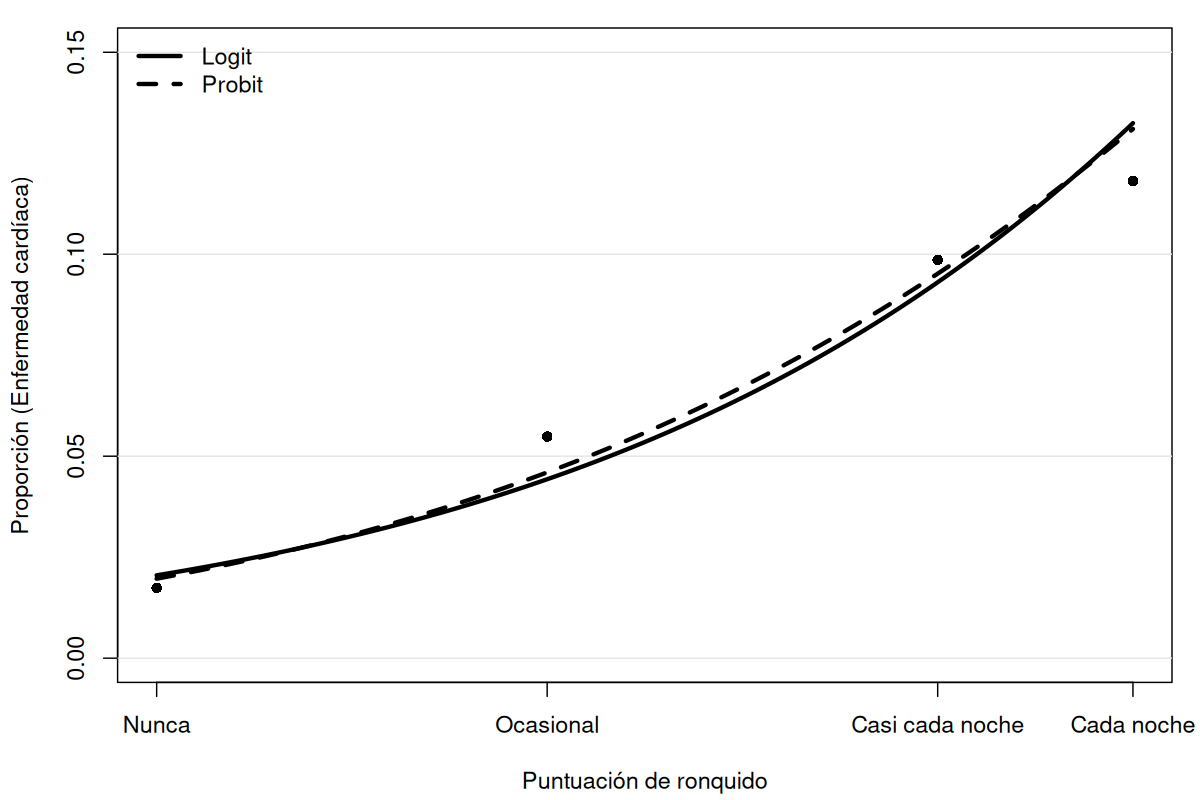
\includegraphics[width=0.7\textwidth]{images/snoring_glm_curves.png}
    \caption{Curvas de probabilidad ajustadas (logit y probit).}
    \label{fig:3}
\end{figure}

La figura confirma la relación positiva y monótona entre la puntuación de ronquido y la probabilidad de padecer una enfermedad cardíaca, evidenciada por la clara tendencia ascendente tanto de los datos como de las curvas. Asimismo, se observa un excelente ajuste de ambos modelos. La superposición casi perfecta de las dos curvas demuestra visualmente la conclusión del análisis: los modelos logit y probit ofrecen resultados prácticamente idénticos y son igualmente efectivos para describir la relación en este conjunto de datos.

\newpage
%%%%%%%%%%%%%%%%%%%%%%%%%%%%%%%%%%%%%%%%%%%%%%%%%%%%%%%%%%%%%%%%%%%%%%%%%%

\section*{Problema \textcolor{CIMATRed}{2}}

Entre los cangrejos cacerola se sabe que cada hembra tiene un macho en su nido, pero puede tener más machos concubinos.

Se considera que la variable respuesta es el número de concubinos y las variables explicativas son: color, estado de la espina central, peso y anchura del caparazón.

\begin{center}
\begin{tabular}{ccccc}
\toprule
\textbf{color} & \textbf{Spine} & \textbf{Width} & \textbf{Satellite} & \textbf{Weight} \\
\midrule
3 & 3 & 28.3 & 8 & 3050 \\
4 & 3 & 22.5 & 0 & 1550 \\
2 & 1 & 26.0 & 9 & 2300 \\
4 & 3 & 24.8 & 0 & 2100 \\
4 & 3 & 26.0 & 4 & 2600 \\
3 & 3 & 23.8 & 0 & 2100 \\
2 & 1 & 26.5 & 0 & 2350 \\
\bottomrule
\end{tabular}
\end{center}

Realizar e interpretar los resultados de ajustar un modelo lineal generalizado tipo \textbf{poisson}.\\

\noindent\fbox{\textbf{SOLUCIÓN}}\\

\textit{Se utilizo el lenguaje de programación \texttt{R} para resolver este problema, el código utilizado se encuentran al final del documento en el apéndice} \textbf{A.2}

Tras ajustar un GLM de tipo Poisson para predecir el número de machos satélite el proceso de ajuste presentó problemas críticos de convergencia e inestabilidad. Los resultados numéricos del ajuste se muestran a continuación: 

\begin{table}[H]
\centering
\caption{Resumen del auste del modelo Poisson}
\label{tab:poisson_summary_invalid}
\begin{tabular}{lrrrr}
\hline
\textbf{Predictor} & \textbf{Estimate} & \textbf{Std. Error} & \textbf{z value} & \textbf{Pr($>$$|$z$|$)} \\
\hline
(Intercept) & $1.40 \times 10^{3}$  & $1.97 \times 10^{6}$  & 0.001 & 0.999 \\
color3      & $-1.42 \times 10^{2}$ & $2.12 \times 10^{5}$  & -0.001 & 0.999 \\
color4      & $-1.47 \times 10^{2}$ & $2.01 \times 10^{5}$  & -0.001 & 0.999 \\
Spine3      & NA                    & NA                    & NA    & NA    \\
Width       & $-9.68 \times 10^{1}$ & $1.33 \times 10^{5}$  & -0.001 & 0.999 \\
Weight      & $4.87 \times 10^{-1}$ & $6.70 \times 10^{2}$  & 0.001 & 0.999 \\
\hline
\multicolumn{5}{l}{\footnotesize Nota: 1 coeficiente (Spine3) no definido por singularidades.} \\
\multicolumn{5}{l}{\footnotesize Parámetro de dispersión para la familia Poisson tomado como 1.} \\
\multicolumn{5}{l}{\footnotesize Devianza Nula: 37.77 con 6 g.l.} \\
\multicolumn{5}{l}{\footnotesize Devianza Residual: $6.69 \times 10^{-10}$ con 2 g.l.} \\
\multicolumn{5}{l}{\footnotesize AIC: 21.258} \\
\multicolumn{5}{l}{\footnotesize Iteraciones de Fisher Scoring: 25} \\
\end{tabular}
\end{table}


Analizando estos resultados, el resumen del modelo poisson nos muestra múltiples indicadores de que el modelo ha fallado, puesto que:

\begin{enumerate}
    \item \textbf{Singularidad y Coeficientes NA:} La nota al pie de la tabla y la fila para \texttt{Spine3} indican una singularidad. Esto se debe a una multicolinealidad perfecta en la muestra de datos (todos los cangrejos con \texttt{Spine=1} también tienen \texttt{color=2}), lo que impide al modelo estimar el efecto de \texttt{Spine3} de forma independiente.

    \item \textbf{Estimaciones y Errores Estándar:} Los valores en las columnas \texttt{Estimate} y \texttt{Std. Error} son extremadamente grandes. Por ejemplo, el intercepto tiene un error estándar de $1.97 \times 10^6$. Errores estándar de esta magnitud nos indican que las estimaciones de los coeficientes no tienen ninguna precisión y son completamente inestables.

    \item \textbf{Significancia Estadística:} Como consecuencia de los enormes errores estándar, todos los valores en la columna \texttt{z value} son casi cero y los $p$-valores son efectivamente 1. Esto confirma que ninguna variable puede ser considerada estadísticamente significativa, no porque no tengan un efecto, sino porque el modelo fue incapaz de estimarlo.

    \item \textbf{Devianza Residual:} La devianza residual es prácticamente cero, $6.69 \times 10^{-10}$, lo que es un síntoma claro de un sobreajuste (overfitting) severo. El modelo se ha ajustado de manera casi perfecta a los 7 puntos de datos, perdiendo toda capacidad de generalización.
\end{enumerate}

\tcbset{colframe=red, colback=white, boxrule=0.3mm, arc=0mm}
\begin{tcolorbox}
Por lo tanto, el modelo es estadísticamente inválido. La causa principal es el tamaño de muestra extremadamente pequeño, n=7, en relación con el número de predictores, lo que provoca multicolinealidad e inestabilidad numérica. Por lo tanto, no es posible extraer ninguna conclusión fiable sobre la relación entre las variables predictoras y el número de machos satélite a partir de este análisis. Adicionalmente, el alto número de iteraciones de Fisher (25) y las advertencias de \texttt{R} sobre la falta de convergencia confirman el fallo del ajuste.
\end{tcolorbox}

\newpage
%%%%%%%%%%%%%%%%%%%%%%%%%%%%%%%%%%%%%%%%%%%%%%%%%%%%%%%%%%%%%%%%%%%%%%%%%%

\section*{Problema \textcolor{CIMATRed}{3}}

Cuando usamos un modelo de regresión logística para clasificación, tenemos que definir el umbral, $p$, a partir del cual declaramos un ``positivo''.

Las curvas ROC grafican las tasas \textit{TPR} vs \textit{FPR} para diferentes umbrales $p$.

\[
TPR = \text{True Positive Rate} = \frac{TP}{P} = \text{``sensitividad''}
\]
\[
FPR = \text{False Positive Rate} = \frac{FP}{N} = 1 - \text{``especificidad''}
\]

\begin{center}
\begin{tabular}{lcc}
\toprule
 & \multicolumn{2}{c}{\textbf{Observados}} \\
\cmidrule(lr){2-3}
\textbf{Decisión} & \textbf{1} & \textbf{0} \\
\midrule
\textbf{\quad\quad 1} & TP & FP \\
\textbf{\quad\quad 0} & FN & TN \\
\midrule
\textbf{Total} & P & N \\
\bottomrule
\end{tabular}
\end{center}

\begin{itemize}
    \item La gráfica de \textit{TPR} vs \textit{FPR} puede interpretarse como una gráfica de ``poder'' vs ``error tipo I''.
    
    \item Idealmente, una regla de decisión estaría en el punto $(0, 1)$.
    
    \item El área bajo la curva, \textit{AUC}, puede verse, es la probabilidad de que un individuo de los positivos, tomado al azar, tenga un riesgo estimado mayor que un individuo de los negativos, tomado al azar.
    
    \item El estadístico $J$ de Youden, es una medida que, con un sólo número, trata de capturar el desempeño de una prueba de diagnóstico. Es la máxima distancia vertical, entre la diagonal y la curva ROC, o equivalentemente
    \[
    J = \text{sensitividad} - (1 - \text{especificidad})
    \]
\end{itemize}

Construyan la curva ROC para el problema de daño coronario y su relación con la edad visto en la clase 3 del curso.

\begin{lstlisting}[language=R, caption={Datos de Edad y Daño Coronario}]
# Hosmer, D.W. & Lemeshow, S.(1989) Applied logistic regression. Wiley
# Edad y Coronaria (daño significativo en coronaria)

edad <- c(
  20, 23, 24, 25, 25, 26, 26, 28, 28, 29, 30, 30, 30, 30, 30, 30, 32, 32, 33, 33,
  34, 34, 34, 34, 34, 35, 35, 36, 36, 36, 37, 37, 37, 38, 38, 39, 39, 40, 40, 41,
  41, 42, 42, 42, 42, 43, 43, 43, 44, 44, 44, 44, 45, 45, 46, 46, 47, 47, 47, 48,
  48, 48, 49, 49, 49, 50, 50, 51, 52, 52, 53, 53, 54, 55, 55, 55, 56, 56, 56, 57,
  57, 57, 57, 57, 57, 58, 58, 58, 59, 59, 60, 60, 61, 62, 62, 63, 64, 64, 65, 69
)

coro <- c(
  0,0,0,0,1,0,0,0,0,0,0,0,0,0,0,1,0,0,0,0,0,1,0,0,0,0,1,0,0,1,0,0,1,0,1,0,1,0,1,0,
  0,0,0,1,0,0,1,0,0,1,1,0,1,0,1,0,0,1,1,0,1,0,0,1,1,1,1,0,1,1,1,1,0,0,1,1,1,1,0,
  1,1,1,1,0,1,1,1,1,1,0,1,1,1
)
\end{lstlisting}

\newpage
\noindent\fbox{\textbf{SOLUCIÓN}}\\

\textit{Se utilizo el lenguaje de programación \texttt{R} para resolver este problema, el código utilizado se encuentran al final del documento en el apéndice} \textbf{A.3}

Buscamos construir y analizar la curva ROC para un modelo que prediga la probabilidad de daño coronario significativo a partir de la edad de un paciente, básicamente la curva ROC nos servirá como herramienta gráfica para evaluar el rendimiento de un clasificador binario a medida que se varía el umbral de discriminación. 

Para este problema se nos pide ajustar un modelo de regresión logística binomial para predecir la probabilidad de daño coronario, $y=1$, a partir de la edad. El modelo tiene la forma:
\begin{equation}
    \log\left(\frac{p}{1-p}\right) = \beta_0 + \beta_1 \cdot \text{edad}
\end{equation}

donde $p = P(y=1 | \text{edad})$. Para la construcción de la curva ROC se generaron las probabilidades predichas $\hat{p}$ para cada observación. Se evaluó un conjunto de umbrales de decisión $t$ sobre estas probabilidades. Para cada umbral, se clasificó una observación como positiva si $\hat{p} \ge t$ y se calcularon los correspondientes valores de TPR y FPR para construir la curva. El área bajo la curva (AUC) se calculó numéricamente utilizando la regla del trapecio. La curva ROC obtenida se muestra a continuación:

\begin{figure}[H]
    \centering
    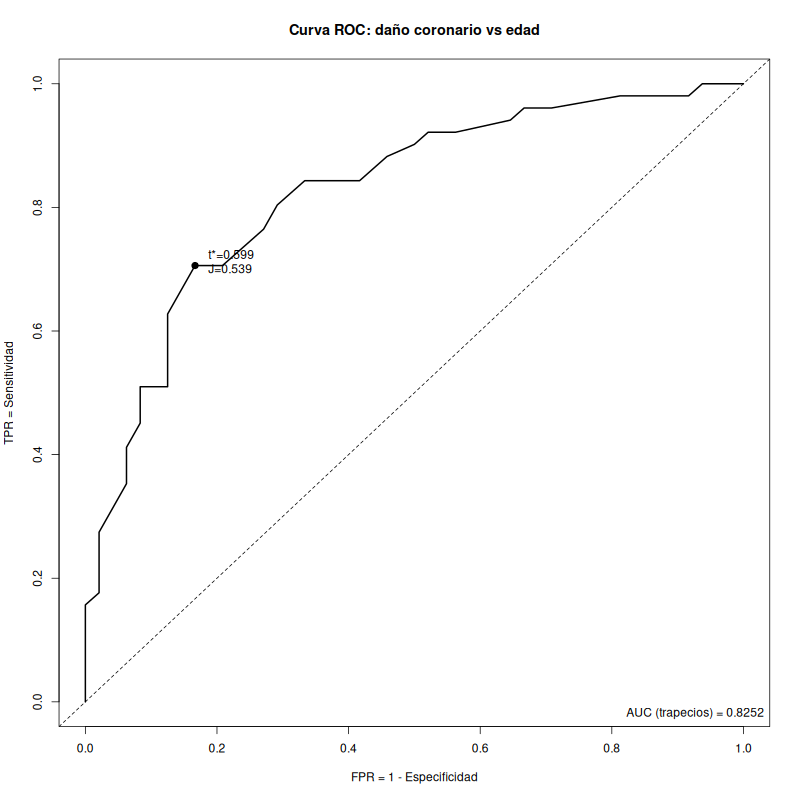
\includegraphics[width=0.65\textwidth]{images/roc_coro.png}
    \caption{Curva ROC para el modelo de daño coronario vs. edad. Se muestra el punto óptimo según el índice $J$ de Youden y el valor del AUC.}
    \label{fig:roc}
\end{figure}

Podemos observar que el modelo de regresión logística demostró una buena capacidad de discriminación. El área bajo la curva calculada fue de \textbf{AUC = 0.8252}, lo que nos indica un buen rendimiento del clasificador (considerando que un valor de 0.5 corresponde al azar y 1.0 a una clasificación perfecta).

Para determinar el umbral optimo $t^*$ se maximizo el estadístico $J$ de Youden y se obtuvo que $\mathbf{t^* = 0.5992}$, este umbral representa el punto de corte en la probabilidad predicha que ofrece el mejor equilibrio entre sensitividad y especificidad. Las métricas de rendimiento en este punto óptimo son:

\begin{itemize}
    \item \textbf{Índice J de Youden máximo:} $J_{max} = 0.5392$
    \item \textbf{Sensitividad (TPR):} $0.7059$
    \item \textbf{Especificidad:} $0.8333$
    \item \textbf{Tasa de Falsos Positivos (FPR):} $0.1667$
\end{itemize}

Al aplicar el umbral óptimo $t^*=0.5992$ a los datos, se obtuvo la siguiente matriz de confusión:

\begin{table}[H]
    \centering
    \caption{Matriz de confusión en el umbral óptimo}
    \label{tab:confusion_matrix}
    \begin{tabular}{lcc}
        \toprule
        & \multicolumn{2}{c}{\textbf{Observados}} \\
        \cmidrule(lr){2-3}
        \textbf{Decisión} & \textbf{1 (Positivo)} & \textbf{0 (Negativo)} \\
        \midrule
        \textbf{1 (Positivo)} & 36 (TP) & 8 (FP) \\
        \textbf{0 (Negativo)} & 15 (FN) & 40 (TN) \\
        \bottomrule
    \end{tabular}
\end{table}

A partir de lo obtenido en la matriz de confusion, podemos derivar las siguientes métricas globales:

\begin{itemize}
    \item \textbf{Accuracy:} $\quad\displaystyle\frac{36 + 40}{36+8+15+40} = \frac{76}{99} \approx 0.7677 $
    \item \textbf{Precision:} $\quad\displaystyle\frac{36}{36+8} = \frac{36}{44} \approx 0.8182 $
\end{itemize}

\tcbset{colframe=red, colback=white, boxrule=0.3mm, arc=0mm}
\begin{tcolorbox}
Por lo tanto, podemos decir que el modelo de regresión logística basado en la edad es una herramienta útil para discriminar entre pacientes con y sin daño coronario, como lo demuestra un AUC de 0.8252. El umbral de probabilidad óptimo de 0.5992 permite clasificar a los pacientes con una sensitividad del 70.6\% y una especificidad del 83.3\%. Esto significa que el modelo, con este punto de corte, identifica correctamente al 70.6\% de los enfermos, mientras que clasifica correctamente al 83.3\% de los sanos. La precisión del 81.8\% indica que, de todos los pacientes clasificados como positivos, la gran mayoría lo son realmente.
\end{tcolorbox}

\newpage
%%%%%%%%%%%%%%%%%%%%%%%%%%%%%%%%%%%%%%%%%%%%%%%%%%%%%%%%%%%%%%%%%%%%%%%%%%

\section*{Problema \textcolor{CIMATRed}{4}}

Los datos de la tabla en la siguiente hoja son números, \textit{n}, de pólizas de seguros y los correspondientes números, \textit{y}, de reclamos (esto es, número de accidentes en los que se pidió el amparo de la póliza). La variable \textit{CAR} es una codificación de varias clases de carros, \textit{EDAD} es la edad del titular de la póliza y \textit{DIST} es el distrito donde vive el titular.

\begin{enumerate}[label=\alph*.]
    \item Calcule la tasa de reclamos, $y/n$, para cada categoría y grafique estas tasas contra las diferentes variables para tener una idea de los efectos principales.
    
    \item Use regresión logística para estimar los efectos principales (cada variable tratada como categórica y modelada usando variables indicadoras) así como sus interacciones.
    
    \item Basados en los resultados del inciso anterior, los autores del artículo donde aparecieron estos datos, decidieron que ninguna interacción era importante y que podían considerar que \textit{CAR} y \textit{EDAD} fuesen tratadas como variables continuas. Ajuste un modelo incorporando estas observaciones y compárelo con el obtenido en (b). ¿Cuáles son las conclusiones?.
\end{enumerate}

\begin{table}[h!]
\centering
\begin{tabular}{cc rrrr}
\toprule
& & \multicolumn{2}{c}{\textbf{DIST = 0}} & \multicolumn{2}{c}{\textbf{DIST = 1}} \\
\cmidrule(lr){3-4} \cmidrule(lr){5-6}
\textbf{CAR} & \textbf{EDAD} & \textit{y} & \textit{n} & \textit{y} & \textit{n} \\
\midrule
1 & 1 & 65 & 317 & 2 & 20 \\
1 & 2 & 65 & 476 & 5 & 33 \\
1 & 3 & 52 & 486 & 4 & 40 \\
1 & 4 & 310 & 3259 & 36 & 316 \\
\addlinespace % Añade un pequeño espacio para separar bloques
2 & 1 & 98 & 486 & 7 & 31 \\
2 & 2 & 159 & 1004 & 10 & 81 \\
2 & 3 & 175 & 1355 & 22 & 122 \\
2 & 4 & 877 & 7660 & 102 & 724 \\
\addlinespace
3 & 1 & 41 & 223 & 5 & 18 \\
3 & 2 & 117 & 539 & 7 & 39 \\
3 & 3 & 137 & 697 & 16 & 68 \\
3 & 4 & 477 & 3442 & 63 & 344 \\
\addlinespace
4 & 1 & 11 & 40 & 0 & 3 \\
4 & 2 & 35 & 148 & 6 & 16 \\
4 & 3 & 39 & 214 & 8 & 25 \\
4 & 4 & 167 & 1019 & 33 & 114 \\
\bottomrule
\end{tabular}
\caption{Tabla de Pólizas de Seguros y Reclamos.}
\label{tab:seguros}
\end{table}

\noindent\fbox{\textbf{SOLUCIÓN}}\\

\textit{Se utilizo el lenguaje de programación \texttt{R} para resolver este problema, el código utilizado se encuentran al final del documento en el apéndice} \textbf{A.5}

Buscamos modelar la tasa de reclamos utilizando un modelo de regresión logística, considerando como variables explicativas el tipo de carro (\textit{CAR}), el grupo de edad del titular (\textit{EDAD}) y el distrito de residencia (\textit{DIST}). Para ello debemos evaluar dos modelos, uno completo con todas las interacciones posibles y un modelo simplificado con solo efectos principales, para determinar cuál de ellos explica mejor la variabilidad en los datos de forma más parsimoniosa.

\newpage
\textbf{a)} Primero, calculamos las tasas de reclamo $y/n$ para cada combinación de las variables categóricas y se generaron gráficos de cajas para visualizar la relación entre la tasa de reclamos y cada una de las variables predictoras como se muestra a continuacion:

\begin{figure}[H]
    \centering
    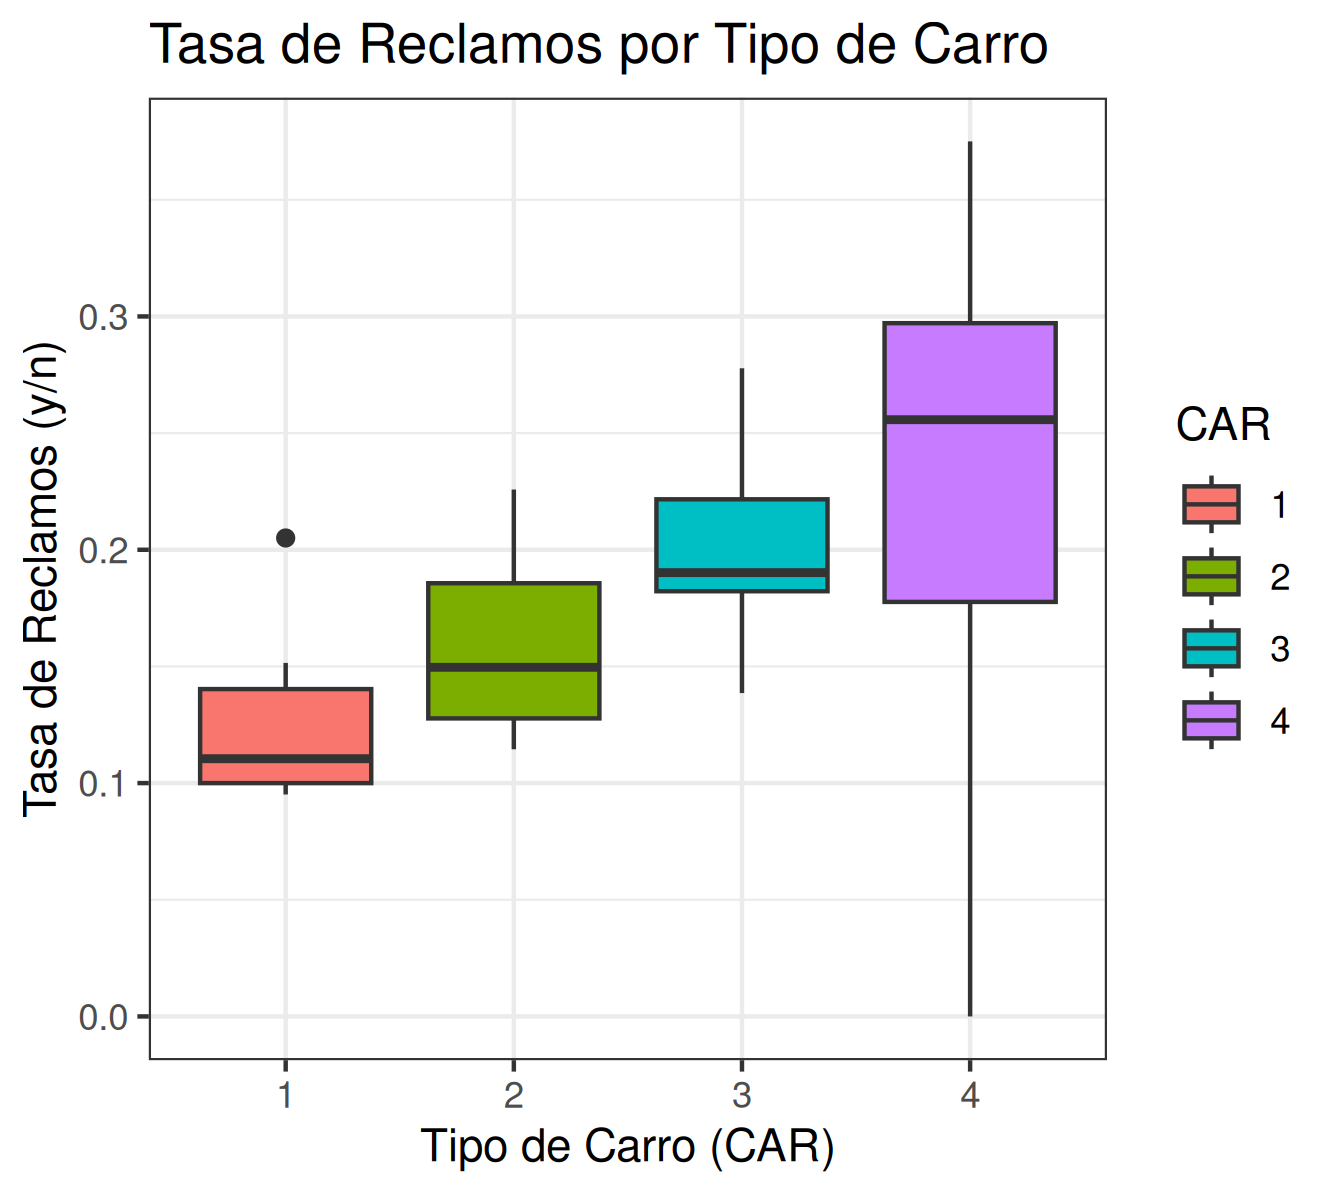
\includegraphics[width=0.5\textwidth]{images/rate_vs_car.png}
    \caption{Tasa de Reclamos por tipo de carro.}
    \label{fig:car_boxplot}
\end{figure}

En la Figura 0.6 se observa una tendencia positiva pues a medida que aumenta la categoría del carro, la mediana y la dispersión de la tasa de reclamos también tienden a aumentar, esto nos sugiere que los carros de categorías superiores están asociados a un mayor riesgo.

\begin{figure}[H]
    \centering
    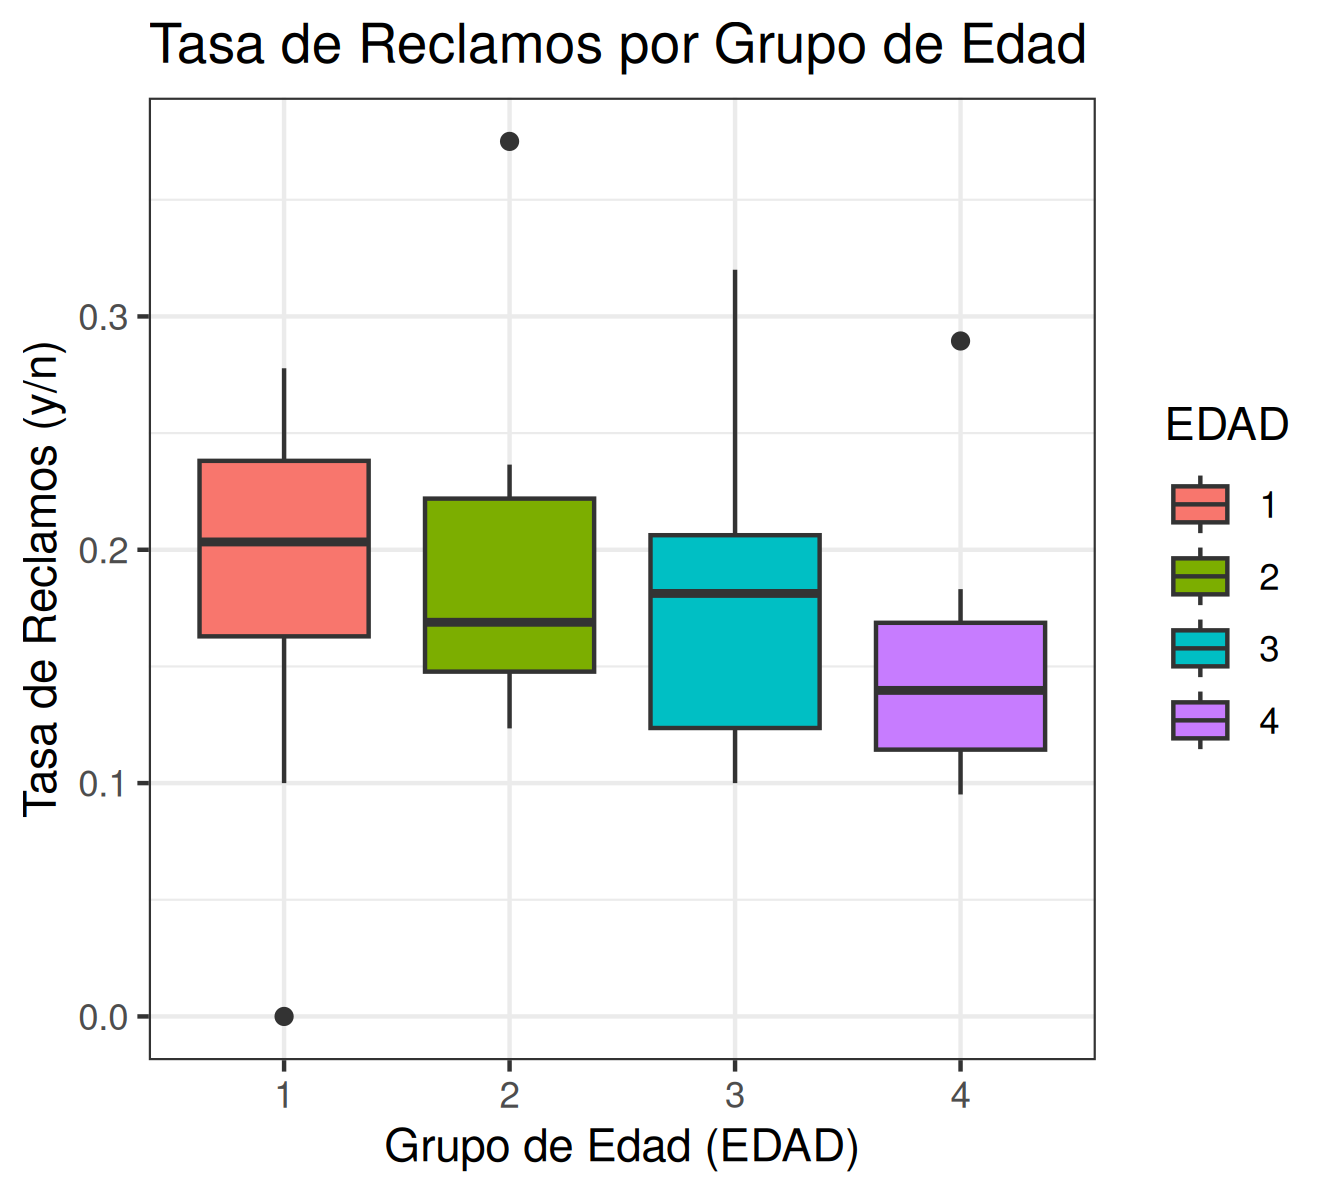
\includegraphics[width=0.5\textwidth]{images/rate_vs_edad.png}
    \caption{Tasa de Reclamos por Grupo de Edad.} 
    \label{fig:edad_boxplot}
\end{figure}

En la Figura 0.7 el gráfico muestra una clara tendencia decreciente. Los grupos de edad más jóvenes (especialmente el grupo 1) presentan las tasas de reclamo más altas. La tasa disminuye consistentemente a medida que aumenta la edad, indicando que la edad es un factor protector.

\begin{figure}[H]
    \centering
    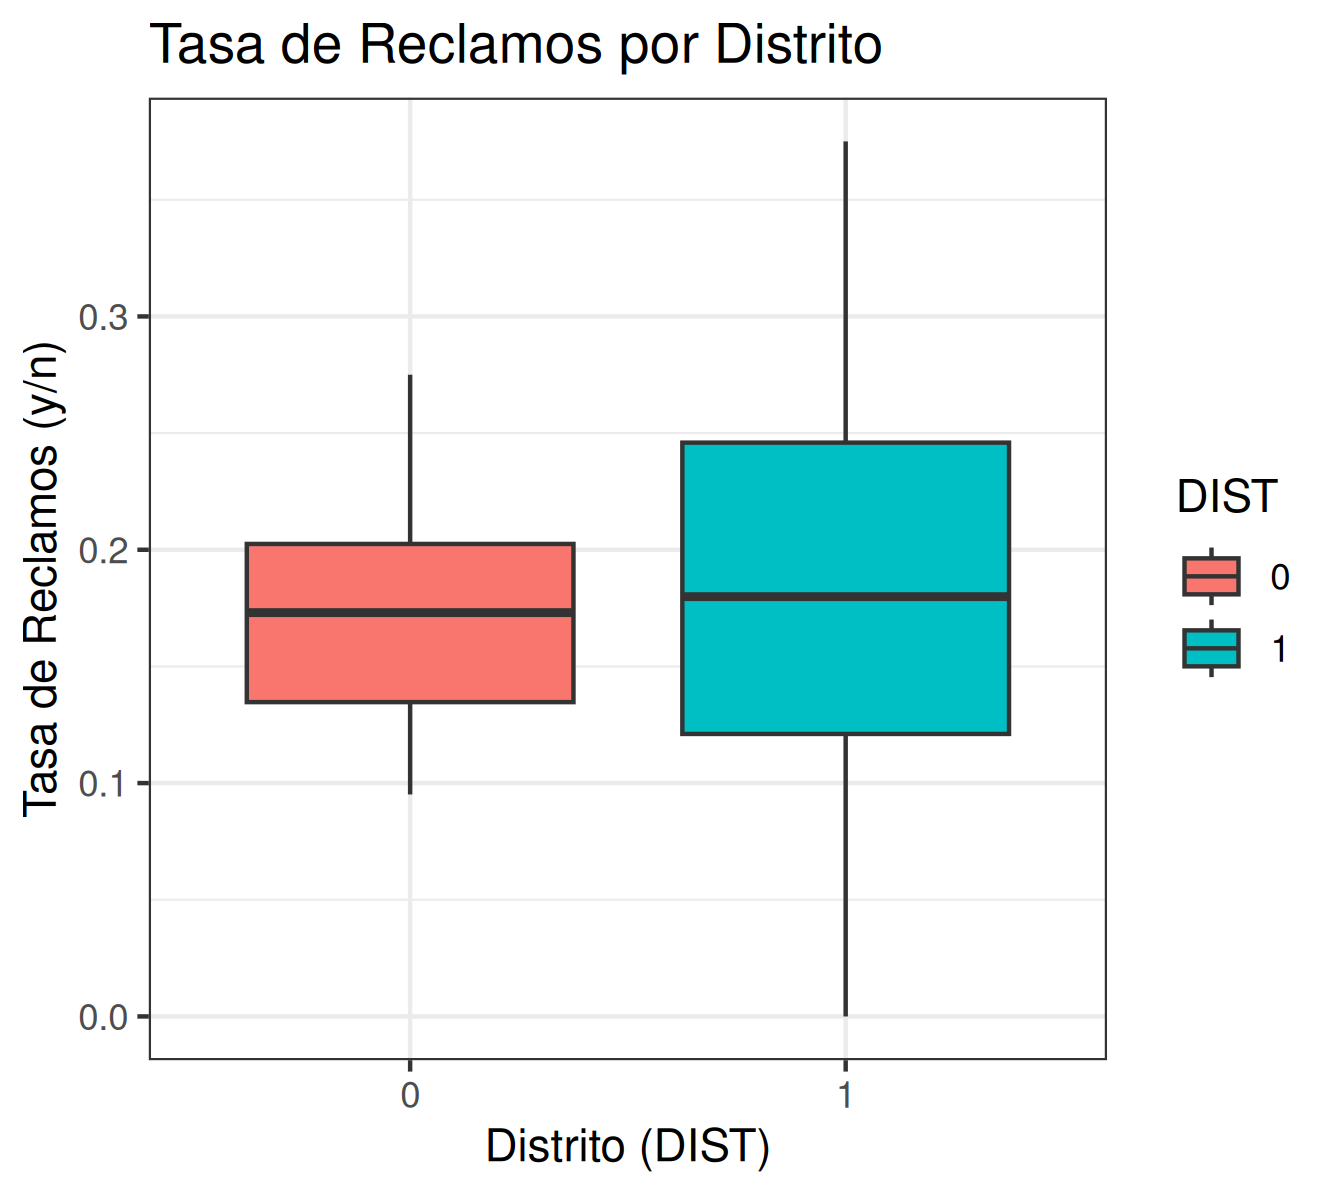
\includegraphics[width=0.5\textwidth]{images/rate_vs_dist.png}
    \caption{Tasa de Reclamos por Distrito}
    \label{fig:dist_boxplot}
\end{figure}

Por ultimo en la Figura 0.8 se aprecia una diferencia notable entre los dos distritos. El distrito 0 presenta tasas de reclamo con una mediana más baja en comparación con el distrito 1, lo que indica que la ubicación geográfica es un predictor potencialmente importante.

\newpage
\textbf{b)} Se ajustó un primer GLM binomial con función de enlace logística. Este modelo incluyó todos los efectos principales y todas las interacciones de segundo y tercer orden entre \textit{CAR}, \textit{EDAD} y \textit{DIST}, tratadas como variables categóricas. El resumen del ajuste se presenta a continuacion: 

\begin{table}[H]
\centering
\caption{Resumen del modelo Logístico completo con interacciones}
\label{tab:modelo_completo}
\footnotesize % Hacemos la fuente un poco más pequeña para que quepa bien
\begin{tabular}{lrrrr}
\toprule
\textbf{Predictor} & \textbf{Estimate} & \textbf{Std. Error} & \textbf{z value} & \textbf{Pr($\mathbf{>|z|}$)} \\
\midrule
(Intercept)        & -1.3550 & 0.1391 & -9.740 & $<2 \times 10^{-16}$$^{***}$ \\
CAR2               & -0.0210 & 0.1793 & -0.117 & 0.906760 \\
CAR3               & -0.1354 & 0.2219 & -0.610 & 0.541753 \\
CAR4               & 0.3856  & 0.3805 & 1.014  & 0.310756 \\
EDAD2              & -0.4892 & 0.1928 & -2.537 & 0.011174$^{*}$ \\
EDAD3              & -0.7668 & 0.2022 & -3.792 & 0.000149$^{***}$ \\
EDAD4              & -0.8976 & 0.1514 & -5.929 & $3.04 \times 10^{-9}$$^{***}$ \\
DIST1              & -0.8422 & 0.7582 & -1.111 & 0.266686 \\
CAR2:EDAD2         & 0.1948  & 0.2396 & 0.813  & 0.416346 \\
CAR3:EDAD2         & 0.6968  & 0.2792 & 2.495  & 0.012586$^{*}$ \\
CAR4:EDAD2         & 0.2865  & 0.4472 & 0.641  & 0.521707 \\
CAR2:EDAD3         & 0.2343  & 0.2454 & 0.955  & 0.339707 \\
CAR3:EDAD3         & 0.8492  & 0.2826 & 3.005  & 0.002654$^{**}$ \\
CAR4:EDAD3         & 0.2349  & 0.4446 & 0.528  & 0.597177 \\
CAR2:EDAD4         & 0.2280  & 0.1923 & 1.185  & 0.235856 \\
CAR3:EDAD4         & 0.5609  & 0.2350 & 2.387  & 0.017001$^{*}$ \\
CAR4:EDAD4         & 0.2374  & 0.3943 & 0.602  & 0.547094 \\
CAR2:DIST1         & 0.9861  & 0.8788 & 1.122  & 0.261808 \\
CAR3:DIST1         & 1.3771  & 0.9390 & 1.467  & 0.142493 \\
CAR4:DIST1         & -21.3479& 37437.8581& -0.001 & 0.999545 \\
EDAD2:DIST1        & 0.9636  & 0.9102 & 1.059  & 0.289733 \\
EDAD3:DIST1        & 0.7668  & 0.9350 & 0.820  & 0.412179 \\
EDAD4:DIST1        & 1.0436  & 0.7809 & 1.336  & 0.181439 \\
CAR2:EDAD2:DIST1   & -1.3972 & 1.0711 & -1.304 & 0.192095 \\
CAR3:EDAD2:DIST1   & -1.7355 & 1.1490 & -1.510 & 0.130932 \\
CAR4:EDAD2:DIST1   & 21.8877 & 37437.8581& 0.001  & 0.999534 \\
CAR2:EDAD3:DIST1   & -0.5163 & 1.0647 & -0.485 & 0.627725 \\
CAR3:EDAD3:DIST1   & -1.0724 & 1.1278 & -0.951 & 0.341658 \\
CAR4:EDAD3:DIST1   & 22.1708 & 37437.8581& 0.001  & 0.999527 \\
CAR2:EDAD4:DIST1   & -0.9497 & 0.9054 & -1.049 & 0.294206 \\
CAR3:EDAD4:DIST1   & -1.2466 & 0.9688 & -1.287 & 0.198168 \\
CAR4:EDAD4:DIST1   & 21.8782 & 37437.8581& 0.001  & 0.999534 \\
\midrule
\multicolumn{5}{l}{\footnotesize Signif. codes: $^{***}0.001$, $^{**}0.01$, $^{*}0.05$} \\
\multicolumn{5}{l}{\footnotesize Null deviance: 244.33 on 31 d.f.} \\
\multicolumn{5}{l}{\footnotesize Residual deviance: $5.26 \times 10^{-10}$ on 0 d.f.} \\
\multicolumn{5}{l}{\footnotesize AIC: 225.92} \\
\end{tabular}
\end{table}

Podemos observar que la mayoría de los términos de interacción no son estadísticamente significativos,  Pr($>|z|) > 0.05$. Además, algunos coeficientes presentan errores estándar extremadamente grandes, por ejemplo \texttt{CAR4:DIST1}), lo que sugiere problemas de inestabilidad o cuasi-separación en el modelo. Este resultado indica que el modelo está sobreajustado y es innecesariamente complejo.

\newpage
\textbf{c)} De acuerdo a los resultados anteriores, se ajustó un segundo modelo más parsimonioso. En este caso, las variables \textit{CAR} y \textit{EDAD} se trataron como continuas (numéricas) y solo se incluyeron los efectos principales, sin interacciones. El resumen del ajuste se muestra a continuación:

\begin{table}[H]
\centering
\caption{Resumen del modelo Logístico simplificado de efectos principales}
\label{tab:modelo_simple}
\begin{tabular}{lrrrr}
\toprule
\textbf{Predictor} & \textbf{Estimate} & \textbf{Std. Error} & \textbf{z value} & \textbf{Pr($\mathbf{>|z|}$)} \\
\midrule
(Intercept) & -1.66749 & 0.08748 & -19.061 & $<2 \times 10^{-16}$$^{***}$ \\
\textbf{CAR}         &  0.23168 & 0.02266 &  10.225 & $<2 \times 10^{-16}$$^{***}$ \\
\textbf{EDAD}        & -0.20967 & 0.02040 & -10.278 & $<2 \times 10^{-16}$$^{***}$ \\
\textbf{DIST1}       &  0.25891 & 0.06420 &   4.033 & $5.5 \times 10^{-5}$$^{***}$ \\
\midrule
\multicolumn{5}{l}{\footnotesize Signif. codes: $^{***}0.001$} \\
\multicolumn{5}{l}{\footnotesize Null deviance: 244.327 on 31 d.f.} \\
\multicolumn{5}{l}{\footnotesize Residual deviance: 30.086 on 28 d.f.} \\
\multicolumn{5}{l}{\footnotesize AIC: 200.01} \\
\end{tabular}
\end{table}

En este modelo, todos los predictores son altamente significativos, por cada incremento en una unidad en la categoría del carro, el log-odds de un reclamo aumenta en 0.232, por cada incremento en una unidad en el grupo de edad, el log-odds de un reclamo disminuye en 0.210 y el log-odds de un reclamo en el distrito 1 es 0.259 mayor que en el distrito 0 (el nivel de referencia).

Para comparar formalmente ambos modelos, se utilizó un test de razón de verosimilitud (ANOVA). La hipótesis nula de esta prueba es que el modelo simple es suficiente para describir los datos, los resultados obtenidos se muestran a continuación: 

\begin{table}[H]
\centering
\caption{Comparación de modelos mediante Test de Razón de Verosimilitud (ANOVA)}
\label{tab:anova}
\begin{tabular}{lrrrrr}
\toprule
Model & Resid. Df & Resid. Dev & Df & Deviance & Pr($>$Chi) \\
\midrule
Simple      & 28 & 30.086 &    &        &         \\
Completo    & 0  & 0.000  & 28 & 30.086 & 0.3591  \\
\bottomrule
\end{tabular}
\end{table}

Podemos ver que el $p$-valor de la prueba es de $0.3591$, el cual es considerablemente mayor que el nivel de significancia de $0.05$, por lo tanto, no se rechaza la hipótesis nula, esto nos indica que los términos de interacción y la complejización del modelo completo no aportan una mejora estadísticamente significativa al ajuste. Adicionalmente, el Criterio de Información de Akaike (AIC) del modelo simple (AIC = 200.01) es sustancialmente menor que el del modelo completo (AIC = 225.92), lo que favorece fuertemente al modelo más simple.

\tcbset{colframe=red, colback=white, boxrule=0.3mm, arc=0mm}
\begin{tcolorbox}
Por lo tanto, el análisis demuestra que el modelo simplificado de efectos principales es superior al modelo completo con interacciones. Es más fácil de interpretar, más estable y tiene un mejor rendimiento según el criterio AIC, sin una pérdida significativa en la capacidad de ajuste, como lo demuestra el test ANOVA. Las conclusiones del estudio son que la probabilidad de reclamo de un seguro aumenta significativamente con la categoría del carro (\textit{CAR}) y para los residentes del distrito 1, mientras que disminuye a medida que aumenta el grupo de edad (\textit{EDAD}) del titular.
\end{tcolorbox}

\newpage
%%%%%%%%%%%%%%%%%%%%%%%%%%%%%%%%%%%%%%%%%%%%%%%%%%%%%%%%%%%%%%%%%%%%%%%%%%

\section*{Problema \textcolor{CIMATRed}{5}}

A lo largo del curso hemos enfatizado el uso del método de Máxima Verosimilitud para todo lo relacionado con estimación. Consideremos ahora una alternativa: El método de la Mínima Ji-Cuadrada. Suponga que las celdas de una multinomial están parametrizadas en términos de un vector $\boldsymbol{\theta} = (\theta_1, \dots, \theta_s)^T$. El método de la mínima ji-cuadrada (ver Agresti, pág. 611) consiste en estimar $\boldsymbol{\theta}$ mediante aquel valor que minimice el estadístico de Pearson
\[
\chi^2 = \sum \frac{(\text{obs} - \text{esp})^2}{\text{esp}} = \sum_{j=1}^K \frac{(y_j - n\pi_j(\boldsymbol{\theta}))^2}{n\pi_j(\boldsymbol{\theta})}
\]

Considere el siguiente problema. Suponga una población muy grande de objetos que pueden clasificarse en tres categorías, A, B y C. Para estimar las proporciones $\pi_1, \pi_2$ y $\pi_3$ correspondientes a cada una de esas categorías, se efectuó un estudio; se obtuvieron tres muestras de tamaños $n_1, n_2$ y $n_3$ tomadas de la población global, sin embargo, en vez de registrar la frecuencia observada de A's, B's y C's de cada muestra, lo que se hizo fue anotar:
\begin{itemize}
    \item Número de A's en la muestra de tamaño $n_1 = y_1$
    \item Número de B's en la muestra de tamaño $n_2 = y_2$
    \item Número de C's en la muestra de tamaño $n_3 = y_3$
\end{itemize}

Estime $\pi_1, \pi_2$ y $\pi_3$ usando el método de la mínima ji-cuadrada; suponga que $n_1=100, y_1=22$, $n_2=150, y_2=52$, $n_3=200, y_3=77$. Esto es, encuentre $\pi_1, \pi_2$ y $\pi_3$ que minimicen
\begin{equation*}
\frac{(y_1 - n_1\pi_1)^2}{n_1\pi_1} + \frac{[(n_1 - y_1) - n_1(1 - \pi_1)]^2}{n_1(1 - \pi_1)} + 
\dots + \frac{(y_3 - n_3\pi_3)^2}{n_3\pi_3} + \frac{[(n_3 - y_3) - n_3(1 - \pi_3)]^2}{n_3(1 - \pi_3)}
\end{equation*}
con la restricción $\pi_3 = 1 - \pi_1 - \pi_2$ (sugerimos usar directamente \texttt{nlminb} de R).\\

\noindent\fbox{\textbf{SOLUCIÓN}}\\

\textit{Se utilizo el lenguaje de programación \texttt{R} para resolver este problema, el código utilizado se encuentran al final del documento en el apéndice} \textbf{A.6}

De acuerdo a la definicion dada del estadístico $\chi^2$ de Pearson, tenemos que para la categoría A, la contribución al estadístico es:
\begin{equation}
    \chi^2_1 = \frac{(y_1 - n_1\pi_1)^2}{n_1\pi_1} + \frac{((n_1 - y_1) - n_1(1 - \pi_1))^2}{n_1(1 - \pi_1)}
\end{equation}

Simplificando el segundo numerador llegamos a que:
\begin{align*}
    \chi^2_1 &= \frac{(y_1 - n_1\pi_1)^2}{n_1\pi_1} + \frac{(y_1 - n_1\pi_1)^2}{n_1(1-\pi_1)}\\[0.1cm]
    &= (y_1 - n_1\pi_1)^2 \left[ \frac{1}{n_1\pi_1} + \frac{1}{n_1(1 - \pi_1)} \right] \\[0.1cm]
    &= (y_1 - n_1\pi_1)^2 \left[ \frac{1-\pi_1+\pi_1}{n_1\pi_1(1-\pi_1)} \right] \\[0.1cm]
    &= \frac{(y_1 - n_1\pi_1)^2}{n_1\pi_1(1-\pi_1)}
\end{align*}

Generalizando para las tres muestras, la función objetivo completa $Q(\boldsymbol{\pi})$ a minimizar seria:
\begin{equation}
Q(\boldsymbol{\pi}) = \frac{(y_1 - n_1\pi_1)^2}{n_1\pi_1(1-\pi_1)} + \frac{(y_2 - n_2\pi_2)^2}{n_2\pi_2(1-\pi_2)} + \frac{(y_3 - n_3\pi_3)^2}{n_3\pi_3(1-\pi_3)}
\end{equation}

Las proporciones deben sumar 1, siendo la restricción:
\begin{equation*}
    \pi_1 + \pi_2 + \pi_3 = 1 \implies \pi_3 = 1 - \pi_1 - \pi_2
\end{equation*}

Sustituyendo $\pi_3$ en $Q$, obtenemos una función de dos variables:
\begin{equation}
    Q(\pi_1, \pi_2) = \frac{(y_1 - n_1\pi_1)^2}{n_1\pi_1(1-\pi_1)} + \frac{(y_2 - n_2\pi_2)^2}{n_2\pi_2(1-\pi_2)} + \frac{(y_3 - n_3(1 - \pi_1 - \pi_2))^2}{n_3(1 - \pi_1 - \pi_2)(\pi_1 + \pi_2)}
\end{equation}

Esta función es compleja para minimizar analíticamente, por lo que se utilizo optimización numérica mediante la función \texttt{nlminb} en \texttt{R} como se sugiere. El optimizador convergió exitosamente, arrojando los siguientes parámetros:
\begin{equation}
    \hat{\pi}_1 = 0.2443 \quad \text{y} \quad \hat{\pi}_2 = 0.3665
\end{equation}

El valor mínimo del estadístico $\chi^2$ fue de $1.0539$.
Calculamos $\hat{\pi}_3$ a partir de la restricción:
\begin{equation}
    \hat{\pi}_3 = 1 - \hat{\pi}_1 - \hat{\pi}_2 = 1 - 0.2443 - 0.3665 = 0.3892
\end{equation}

Por lo tanto, las proporciones poblacionales estimadas por el método de la Mínima Ji-Cuadrada son:


\begin{center}
\fcolorbox{red}{white}{
    \begin{minipage}{0.45\textwidth} 
    \begin{itemize}
        \item \textbf{Proporción de A ($\hat{\pi}_1$):} 24.43\%
        \item \textbf{Proporción de B ($\hat{\pi}_2$):} 36.65\%
        \item \textbf{Proporción de C ($\hat{\pi}_3$):} 38.92\%
    \end{itemize}
    \end{minipage}
}
\end{center}

\newpage
%%%%%%%%%%%%%%%%%%%%%%%%%%%%%%%%%%%%%%%%%%%%%%%%%%%%%%%%%%%%%%%%%%%%%%%%%%


\section*{Problema \textcolor{CIMATRed}{6}}

Se toman los datos relacionados con el hundimiento del Titanic en abril de 1912. El resultado se puede expresar en una tabla de dimensión 4.

Las variables son \texttt{Class} de los pasajeros (1, 2, 3, Tripulación), \texttt{Sex} de los pasajero (Male, Female), \texttt{Age} de los pasajeros (Child, Adult), y \texttt{Survived} si los pasajeros sobrevivieron o no (No, Yes). Usar librería en R ``titanic'' y los datos se encuentran en la variable ``Titanic''.

\vspace{1em} % Añade un espacio vertical

Considerar entonces un modelo log-lineal para analizar los posibles efectos:
\begin{itemize}
    \item \texttt{Class}: Hay más pasajeros en algunas clases que en otras.
    \item \texttt{Sex}: Hay más pasajeros en un sexo que en otro.
    \item \texttt{Age}: Hay más pasajeros en un grupo de edad que en otro.
    \item \texttt{Survived}: Hay más pasajeros o vivos o muertos que la alternativa.
    \item \texttt{Class} $\times$ \texttt{Sex}: \texttt{Class} y \texttt{Sex} no son independientes.
    \item \texttt{Class} $\times$ \texttt{Age}: \texttt{Class} y \texttt{Age} no son independientes.
    \item \texttt{Class} $\times$ \texttt{Survived}: \texttt{Class} y \texttt{Survived} no son independientes.
    \item \texttt{Sex} $\times$ \texttt{Age}: \texttt{Sex} y \texttt{Age} no son independientes.
    \item \texttt{Sex} $\times$ \texttt{Survived}: \texttt{Sex} y \texttt{Survived} no son independientes.
    \item \texttt{Age} $\times$ \texttt{Survived}: \texttt{Age} y \texttt{Survived} no son independientes.
    \item \texttt{Class} $\times$ \texttt{Sex} $\times$ \texttt{Age}, \texttt{Class} $\times$ \texttt{Sex} $\times$ \texttt{Survived}, \texttt{Class} $\times$ \texttt{Age} $\times$ \texttt{Survived}, \texttt{Sex} $\times$ \texttt{Age} $\times$ \texttt{Survived}: hay interacción triple entre las variables.
    \item \texttt{Class} $\times$ \texttt{Sex} $\times$ \texttt{Age} $\times$ \texttt{Survived}: hay interacción cuádruple entre las variables.
\end{itemize}

\noindent\fbox{\textbf{SOLUCIÓN}}\\

\textit{Se utilizo el lenguaje de programación \texttt{R} para resolver este problema, el código utilizado se encuentran al final del documento en el apéndice} \textbf{A.7}

Buscamos identificar las asociaciones e interacciones significativas entre estas variables para entender los patrones de supervivencia en el desastre del Titanic. Primero se comenzó con el ajuste de un ``modelo saturado", que incluye todos los efectos principales y todas las interacciones posibles hasta el cuarto orden (\texttt{Class} $\times$ \texttt{Sex} $\times$ \texttt{Age} $\times$ \texttt{Survived}). Este modelo se ajusta perfectamente a los datos, como lo indica una devianza residual de prácticamente cero, pero es inherentemente complejo.

Para obtener un modelo más parsimonioso, se utilizó una estrategia de eliminación hacia atrás, comenzando por evaluar la significancia del término de interacción de orden más alto. Se utilizó la función \texttt{drop1()} para realizar un análisis de devianza, cuyos resultados se muestran a continuación:

\begin{table}[H]
\centering
\caption{Análisis de devianza para el modelo saturado}
\label{tab:drop1}
\begin{tabular}{lrrrr}
\toprule
\textbf{Término a eliminar} & \textbf{Df} & \textbf{Devianza} & \textbf{AIC} & \textbf{Pr($>$Chi)} \\
\midrule
$<$none$>$                 &             & 4.46e-10          & 191.4        &                     \\
Class:Sex:Age:Survived      & 3           & 4.24e-10          & 185.4        & 1.000               \\
\bottomrule
\end{tabular}
\end{table}

Podemos observar que el $p$-valor asociado a la interacción de cuarto orden (\texttt{Class:Sex:Age:Survived}) es de $1.0$, lo que indica una falta total de significancia estadística. Esto nos sugiere que cualquier relación entre tres de las variables no cambia a través de los niveles de la cuarta variable, por lo tanto, este término puede ser eliminado del modelo sin una pérdida significativa de ajuste.

Con base en este resultado, se ajustó un segundo modelo que incluye únicamente interacciones de hasta tres vías (\texttt{Model 1}). Para confirmar formalmente que este modelo más simple es suficiente, se comparó con el modelo saturado (\texttt{Model 2}) mediante un test de ANOVA:

\begin{table}[H]
\centering
\caption{Comparación ANOVA de modelos anidados}
\label{tab:anova}
\begin{tabular}{lrrrrr}
\toprule
\textbf{Modelo} & \textbf{Resid. Df} & \textbf{Resid. Dev} & \textbf{Df} & \textbf{Devianza} & \textbf{Pr($>$Chi)} \\
\midrule
1 (3-vías)      & 3                  & 4.24e-10            &             &                   &                     \\
2 (Saturado)    & 0                  & 4.46e-10            & 3           & -2.25e-11         &                     \\
\bottomrule
\end{tabular}
\end{table}

Esta comparación confirma que el modelo saturado no ofrece una mejora significativa sobre el modelo con interacciones de tres vías. Por lo tanto seleccionamos el modelo de interacciones de tres vías como el modelo final por ser el más parsimonioso que describe adecuadamente las relaciones en los datos.

Los coeficientes del modelo final se presentan a continuacion:  

\begin{table}[H]
\centering
\caption{Coeficientes del modelo de interacciones de tres vías}
\label{tab:coefs}
\resizebox{\textwidth}{!}{%
\begin{tabular}{lrrrr}
\toprule
\textbf{Coeficiente} & \textbf{Estimate} & \textbf{Std. Error} & \textbf{z value} & \textbf{Pr($>$$|$z$|$)} \\
\midrule
(Intercept)                     & -2.292e+01 & 5.750e+04 & 0.000 & 0.999682    \\
SexFemale                       & -5.206e+00 & 1.326e+00 & -3.925 & 8.68e-05 ***\\
\addlinespace
Class3rd:SexFemale              & 4.483e+00 & 1.293e+00 & 3.468 & 0.000525 ***\\
SexFemale:SurvivedYes           & 3.596e+00 & 7.478e-01 & 4.809 & 1.52e-06 ***\\
\addlinespace
Class3rd:SexFemale:AgeAdult     & -2.569e+00 & 1.183e+00 & -2.171 & 0.029895 * \\
Class3rd:SexFemale:SurvivedYes  & -2.800e+00 & 5.687e-01 & -4.923 & 8.52e-07 ***\\
\bottomrule
\multicolumn{5}{l}{\footnotesize{Nota: Solo se muestran los términos más relevantes y significativos para la discusión.}} \\
\multicolumn{5}{l}{\footnotesize{Signif. codes:  0 ‘***’ 0.001 ‘**’ 0.01 ‘*’ 0.05 ‘.’ 0.1 ‘ ’ 1}}
\end{tabular}%
}
\end{table}

De la tabla de coeficientes, se extraen las siguientes conclusiones clave:
\begin{itemize}
    \item \textbf{Interacción \texttt{Sex:Survived} (***)}: El término \texttt{SexFemale:SurvivedYes} es altamente significativo. Esto confirma la conocida política de ``mujeres y niños primero", indicando que la probabilidad de supervivencia estaba fuertemente asociada con ser mujer.
    
    \item \textbf{Interacción \texttt{Class:Sex} (***)}: La interacción \texttt{Class3rd:SexFemale} es también significativa. Esto sugiere que la distribución de hombres y mujeres no era homogénea a través de las clases, la proporción de mujeres en tercera clase era diferente a la de primera clase (categoría de referencia).

    \item \textbf{Interacción \texttt{Class:Sex:Survived} (***)}:El término \texttt{Class3rd:SexFemale:SurvivedYes} tambien es altamente significativo. Esto implica que la ventaja de supervivencia para las mujeres (observada en la interacción \texttt{Sex:Survived}) \textbf{no era la misma en todas las clases}. Específicamente, la ventaja de supervivencia de ser mujer era significativamente diferente (en este caso, menor) en la tercera clase en comparación con la primera clase.

    \item \textbf{Interacción \texttt{Class:Sex:Age} (*)}: El término \texttt{Class3rd:SexFemale:AgeAdult} es significativo, lo que indica que la combinación de ser una mujer adulta en tercera clase ocurría con una frecuencia distinta a la que se esperaría si estos factores fueran independientes.
\end{itemize}

\tcbset{colframe=red, colback=white, boxrule=0.3mm, arc=0mm}
\begin{tcolorbox}
Por lo tanto, el análisis log-lineal no solo confirma los efectos principales conocidos (que la clase, el sexo y la edad influyeron en la supervivencia), sino que también cuantifica las complejas interacciones entre ellos. El hallazgo más importante es que los factores no actuaron de forma aislada pues el privilegio de la clase social moduló la ventaja de supervivencia otorgada a las mujeres, pintando un cuadro más matizado de la dinámica social a bordo del Titanic..
\end{tcolorbox}

\newpage
%%%%%%%%%%%%%%%%%%%%%%%%%%%%%%%%%%%%%%%%%%%%%%%%%%%%%%%%%%%%%%%%%%%%%%%%%%

\section*{Problema \textcolor{CIMATRed}{7}}

Se ha realizado un análisis sobre el valor terapéutico del ácido ascórbico (vitamina C) en relación a su efecto sobre la gripe común. Se tiene una tabla $2 \times 2$ con los recuentos correspondientes para una muestra de 279 personas:

\begin{center}
\begin{tabular}{l ccc}
\toprule
& \textbf{Gripe} & \textbf{No Gripe} & \textbf{Totales} \\
\midrule
\textbf{Placebo} & 31 & 109 & 140 \\
\textbf{Ácido Ascórbico} & 17 & 122 & 139 \\
\midrule
\textbf{Totales} & 48 & 231 & 279 \\
\bottomrule
\end{tabular}
\end{center}

Aplicar un modelo lineal para determinar si existe evidencia suficiente para asegurar que el ácido ascórbico ayuda a tener menos gripe.\\

\noindent\fbox{\textbf{SOLUCIÓN}}\\

\textit{Se utilizo el lenguaje de programación \texttt{R} para resolver este problema, el código utilizado se encuentran al final del documento en el apéndice} \textbf{A.8}

Para evaluar la relación entre el tipo de tratamiento y la probabilidad de contraer gripe, se ajustó un GLM con una familia binomial y una función de enlace logística. Sabemos que tiene la forma:
\begin{equation}
    \log\left(\frac{\pi}{1-\pi}\right) = \beta_0 + \beta_1 X_1
\end{equation}

Para este problema particular $\pi$ es la probabilidad de contraer gripe, $\beta_0$ es el log-odds de contraer gripe para el grupo de referencia (placebo), $X_1$ sera la variable indicadora que toma el valor 1 si el tratamiento es ácido ascórbico y 0 si es placebo, por ultimo $\beta_1$ representa el cambio en el log-odds de contraer gripe al pasar del grupo placebo al grupo de ácido ascórbico. Buscamos estimar los coeficientes $\beta_0$ y $\beta_1$ y evaluar si $\beta_1$ es estadísticamente diferente de cero. Al ajustar el modelo de regresión logística a los datos, se obtuvieron los siguientes resultados :

\begin{table}[H]
\centering
\caption{Resumen del ajuste del modelo para el tratamiento}
\label{tab:tratamiento_summary}
\begin{tabular}{lrrrr}
\hline
 & \textbf{Estimate} & \textbf{Std. Error} & \textbf{z value} & \textbf{Pr($\mathbf{>|z|}$)} \\
\hline
\textbf{Intercept}                 & -1.2574 & 0.2035 & -6.177 & $6.53 \times 10^{-10}$$^{***}$ \\
\textbf{TratamientoAcidoAscorbico} & -0.7134 & 0.3293 & -2.166 & $0.0303$$^{*}$ \\
\hline
\multicolumn{5}{l}{\footnotesize Signif. codes: $^{***}0.001$, $^{**}0.01$, $^{*}0.05$, $^{.}0.1$} \\
\multicolumn{5}{l}{\footnotesize Null deviance: 4.8717 on 1 d.f.} \\
\multicolumn{5}{l}{\footnotesize Residual deviance: $7.55 \times 10^{-15}$ on 0 d.f.} \\
\multicolumn{5}{l}{\footnotesize AIC: 13.578} \\
\multicolumn{5}{l}{\footnotesize Fisher Scoring iterations: 3} \\
\end{tabular}
\end{table}

Observamos que se obtuvo un $\hat{\beta}_0 = -1.2574$ y $\hat{\beta}_1 = -0.7134$ este valor indica que el log-odds de contraer gripe para el grupo que tomó ácido ascórbico es 0.7134 unidades menor que el del grupo Placebo. El $p$-valor asociado al coeficiente del tratamiento con ácido ascórbico es \textbf{0.0303}. Dado que este valor es menor que el nivel de significancia estándar, $\alpha = 0.05$, se rechaza la hipótesis nula de que el coeficiente es igual a cero, es decir $H_0: \beta_1 = 0$. Esto implica que el tipo de tratamiento tiene un efecto estadísticamente significativo en la probabilidad de contraer gripe.

Para completar esta interpretación, se calculo el Odds Ratio (OR):
\begin{equation}
    \text{OR} = e^{\hat{\beta}_1} = e^{-0.7134} \approx 0.49
\end{equation}

Un Odds Ratio de \textbf{0.49} nos dice que las odds (chances) de contraer gripe en el grupo que recibió ácido ascórbico son aproximadamente el 49\% de las \textit{odds} del grupo que recibió el placebo. Dicho de otra manera, el tratamiento con ácido ascórbico reduce las odds de contraer gripe en un 51\%.

\tcbset{colframe=red, colback=white, boxrule=0.3mm, arc=0mm}
\begin{tcolorbox}
Por lo tanto, el análisis del GLM nos proporciona \textbf{evidencia estadística suficiente} para asegurar que el ácido ascórbico tiene un efecto protector contra la gripe común en la población estudiada. El efecto es estadísticamente significativo, con $p = 0.0303$, y un Odds Ratio de 0.49 indica que el tratamiento reduce a casi la mitad las ``chances" de enfermarse en comparación con el placebo.
\end{tcolorbox}

\newpage
%%%%%%%%%%%%%%%%%%%%%%%%%%%%%%%%%%%%%%%%%%%%%%%%%%%%%%%%%%%%%%%%%%%%%%%%%%

\appendix  
\section{Código en \textcolor{CIMATRed}{R}}

A continuación, se presentan los scripts de \texttt{R} utilizados para cada uno de los problemas resueltos en este reporte.


\subsection{Problema \textcolor{CIMATRed}{1}}

\begin{lstlisting}[language=R, caption={Script: Ronquido y enfermedad cardiaca}, label={lst:script1}]
# =============================================================================
# Problema 2 
# Script: Ronquido y enfermedad cardíaca
# Autor: Diego Paniagua Molina
# Fecha: 2025-09-18
# =============================================================================

# Carpetas --------------------------------------------------------------------
dir_report   <- file.path("report")
dir_models   <- file.path("report", "models")
dir_figs     <- file.path("report", "figures")

for (d in c(dir_report, dir_models, dir_figs)) {
  if (!dir.exists(d)) dir.create(d, recursive = TRUE, showWarnings = FALSE)
}

# Datos -----------------------------------------------------------------------
snore  <- c("Nunca","Ocasional","Casi cada noche","Cada noche")
score  <- c(0, 2, 4, 5)             # puntuaciones relativas
SI     <- c(24, 35, 21, 30)
NO     <- c(1355,603,192,224)

df <- data.frame(
  snore = factor(snore, levels = snore),  # convierte a factor y preserva orden
  score = score,
  SI    = SI,
  NO    = NO
)
df$tot  <- df$SI + df$NO
df$prop <- df$SI / df$tot

cat("\n=== Datos ===\n")
print(df)

# Modelos GLM: logit y probit -------------------------------------------------
fit_logit  <- glm(cbind(SI, NO) ~ score, data = df,
                  family = binomial(link = "logit"))
fit_probit <- glm(cbind(SI, NO) ~ score, data = df,
                  family = binomial(link = "probit"))

cat("\n=== Resumen LOGIT ===\n")
print(summary(fit_logit))
cat("\n=== Resumen PROBIT ===\n")
print(summary(fit_probit))

# Guardar modelos -------------------------------------------------------------
saveRDS(fit_logit,  file.path(dir_models, "snoring_logit.rds"))
saveRDS(fit_probit, file.path(dir_models, "snoring_probit.rds"))

# Figura: observados vs curvas logit/probit -----------------------------------
png(file.path(dir_figs, "snoring_glm_curves.png"),
    width = 1200, height = 800, res = 140)

op <- par(mar=c(4.2,4.2,1,1))
plot(df$score, df$prop, pch = 16,
     ylim = c(0, max(df$prop, 0.15)),
     xlab = "Puntuación de ronquido",
     ylab = "Proporción (Enfermedad cardíaca)",
     xaxt = "n")
axis(1, at = df$score, labels = df$snore)
abline(h = pretty(c(0, max(df$prop, 0.15))), col = "gray90", lty = 1)

grid_sc <- data.frame(score = seq(0, 5, length.out = 301))
lines(grid_sc$score, predict(fit_logit,  newdata = grid_sc, type = "response"), lwd = 3)
lines(grid_sc$score, predict(fit_probit, newdata = grid_sc, type = "response"), lwd = 3, lty = 2)

legend("topleft", bty = "n", lwd = 3, lty = c(1,2),
       legend = c("Logit", "Probit"))
par(op)
dev.off()

# Mensaje de confirmacion -----------------------------------------------------
cat("\nArchivos generados:\n")
cat(" - Modelos: report/models/snoring_logit.rds, snoring_probit.rds\n")
cat(" - Figura  : report/figures/snoring_glm_curves.png\n\n")

\end{lstlisting}

\clearpage

\subsection{Problema \textcolor{CIMATRed}{2}}

\begin{lstlisting}[language=R, caption={Script: Cangrejos cacerola}, label={lst:script4}]

# =============================================================================
# Problema 3 
# Script: Cangrejos cacerola
# Autor: Diego Paniagua Molina
# Fecha: 2025-09-20
# =============================================================================

# Cargar librerias ------------------------------------------------------------
library(here)
library(dplyr) 

# Datos -----------------------------------------------------------------------
crabs_df <- data.frame(
  color = c(3, 4, 2, 4, 4, 3, 2),
  Spine = c(3, 3, 1, 3, 3, 3, 1),
  Width = c(28.3, 22.5, 26.0, 24.8, 26.0, 23.8, 26.5),
  Satellite = c(8, 0, 9, 0, 4, 0, 0),
  Weight = c(3050, 1550, 2300, 2100, 2600, 2100, 2350)
)

# Preparacion de datos -------------------------------------------------------
# Las variables 'color' y 'Spine' son categóricas. Las convertimos a factores.
crabs_df <- crabs_df %>%
  mutate(
    color = as.factor(color),
    Spine = as.factor(Spine)
  )

print("Estructura de los datos:")
glimpse(crabs_df)

# Ajuste GLM Poisson ----------------------------------------------------------
poisson_model <- glm(Satellite ~ color + Spine + Width + Weight, 
                     data = crabs_df, 
                     family = poisson(link = "log"))

# Guardar resultados ----------------------------------------------------------
model_summary <- summary(poisson_model)

print("Resumen del Modelo de Poisson:")
print(model_summary)

\end{lstlisting}



\clearpage

\subsection{Problema \textcolor{CIMATRed}{3}}

\begin{lstlisting}[language=R, caption={Script: Edad y daño coronario}, label={lst:script4}]

# =============================================================================
# Problema 5
# Script: Edad y daño coronario
# Autor: Diego Paniagua Molina
# Fecha: 2025-09-19
# =============================================================================

# Datos -----------------------------------------------------------------------
edad <- c(
  20, 23, 24, 25, 25, 26, 26, 28, 28, 29, 30, 30, 30, 30, 30, 30, 32, 32, 33, 33, 
  34, 34, 34, 34, 34, 35, 35, 36, 36, 37, 37, 37, 38, 38, 39, 39, 40, 40, 41, 41, 
  42, 42, 42, 42, 43, 43, 43, 44, 44, 44, 44, 45, 45, 46, 46, 47, 47, 47, 48, 48, 
  48, 49, 49, 49, 50, 50, 51, 52, 52, 53, 53, 54, 55, 55, 55, 56, 56, 56, 57, 57, 
  57, 57, 57, 57, 58, 58, 58, 59, 59, 60, 60, 61, 62, 62, 63, 64, 64, 65, 69)

coro <- c(
  0,0,0,0,1,0,0,0,0,0,0,0,0,1,0,0,0,0,0,1,0,0,0,0,1,0,0,1,0,1,0,0,0,1,0,1,0,
  0,0,0,1,0,0,1,0,1,1,0,1,0,1,0,1,0,0,1,0,1,1,1,0,1,1,1,1,1,1,0,
  0,1,1,1,1,0,1,1,1,1,0,1,1,1,1,0,1,1,1,1,1,1,0,1,1,1,1,1,1,1,1)

stopifnot(length(edad) == length(coro))
y <- as.integer(coro)             # 0/1
n <- length(y)
P <- sum(y == 1L)                 # Positivos observados
N <- sum(y == 0L)                 # Negativos observados


# Modelo logístico ------------------------------------------------------------
mod <- glm(y ~ edad, family = binomial)
phat <- as.numeric(predict(mod, type = "response"))

# Curva ROC (barrido de umbrales) ---------------------------------------------
thr_unique <- sort(unique(phat))
thr <- c(Inf, rev(thr_unique), -Inf)   # asegura extremos (0,0) y (1,1)

TPR <- FPR <- SPEC <- SENS <- J <- numeric(length(thr))

for (i in seq_along(thr)) {
  t <- thr[i]
  yhat <- as.integer(phat >= t)
  TP <- sum(yhat == 1L & y == 1L)
  FP <- sum(yhat == 1L & y == 0L)
  TN <- sum(yhat == 0L & y == 0L)
  FN <- sum(yhat == 0L & y == 1L)
  
  SENS[i] <- if (P > 0) TP / P else NA_real_         # TPR
  SPEC[i] <- if (N > 0) TN / N else NA_real_         # Specificity
  TPR[i]  <- SENS[i]
  FPR[i]  <- 1 - SPEC[i]
  
  J[i] <- SENS[i] - (1 - SPEC[i])    # = TPR - FPR = sens + espec - 1
}

# Ordenamos por FPR ascendente (eje x) para AUC con trapecios
ord <- order(FPR, TPR)
FPRo <- FPR[ord]
TPRo <- TPR[ord]

# AUC (regla del trapecio) ----------------------------------------------------
AUC <- sum(diff(FPRo) * (head(TPRo, -1) + tail(TPRo, -1)) / 2)

# Umbral óptimo por Youden J --------------------------------------------------
Jmax <- max(J, na.rm = TRUE)
cand <- which(J == Jmax)

# Elegimos el candidato con menor FPR; si empata, mayor TPR
if (length(cand) > 1L) {
  sub <- cand[order(FPR[cand], -TPR[cand])]
  idx_opt <- sub[1L]
} else {
  idx_opt <- cand
}
t_opt <- thr[idx_opt]
tpr_opt <- TPR[idx_opt]
fpr_opt <- FPR[idx_opt]
spec_opt <- 1 - fpr_opt
sens_opt <- tpr_opt

# Matriz de confusión en t_opt y métricas -------------------------------------
yhat_opt <- as.integer(phat >= t_opt)
TP <- sum(yhat_opt == 1L & y == 1L)
FP <- sum(yhat_opt == 1L & y == 0L)
TN <- sum(yhat_opt == 0L & y == 0L)
FN <- sum(yhat_opt == 0L & y == 1L)

acc  <- (TP + TN) / (P + N)
prec <- if ((TP + FP) > 0) TP / (TP + FP) else NA_real_

# Gráfica ROC -----------------------------------------------------------------
png("results/figures/roc_coro.png", width = 800, height = 800)
plot(FPRo, TPRo, type = "l", lwd = 2,
     xlab = "FPR = 1 - Especificidad",
     ylab = "TPR = Sensitividad",
     main = "Curva ROC: daño coronario vs edad")
abline(0, 1, lty = 2)  # diagonal
points(fpr_opt, tpr_opt, pch = 19, cex = 1.2)
text(fpr_opt, tpr_opt,
     labels = sprintf("  t*=%.3f\n  J=%.3f", t_opt, Jmax),
     pos = 4)
legend("bottomright",
       legend = sprintf("AUC (trapecios) = %.4f", AUC),
       bty = "n")
dev.off()

cat("Imagen guardada en: report/figures/roc_coro.png\n")

# Resumen de resultados -------------------------------------------------------
cat("\n================= RESUMEN =================\n")
cat(sprintf("AUC (trapecios): %.6f\n", AUC))
cat(sprintf("Umbral óptimo (Youden J): t* = %.6f\n", t_opt))
cat(sprintf("  Sensitividad (TPR): %.4f\n", sens_opt))
cat(sprintf("  Especificidad:      %.4f\n", spec_opt))
cat(sprintf("  FPR:                %.4f\n", fpr_opt))
cat(sprintf("  J = TPR - FPR:      %.4f\n", Jmax))

cat("\nMatriz de confusión en t*:\n")
tab <- matrix(c(TP, FP, FN, TN), nrow = 2, byrow = TRUE,
              dimnames = list("Decisión" = c("1", "0"),
                              "Observado" = c("1", "0")))
print(tab)
cat(sprintf("\nAccuracy:  %.4f", acc))
cat(sprintf("\nPrecision: %.4f\n", prec))

\end{lstlisting}


\clearpage

\subsection{Problema \textcolor{CIMATRed}{4}}

\begin{lstlisting}[language=R, caption={Script: Reclamo polizas de seguros.}, label={lst:script8}]

# =============================================================================
# Problema 7 
# Script: Reclamos polizas de seguro
# Autor: Diego Paniagua Molina
# Fecha: 2025-09-20
# =============================================================================

# Librerias -------------------------------------------------------------------
library(here)
library(dplyr)
library(tidyr)
library(ggplot2)

# Dataset ---------------------------------------------------------------------
insurance_wide_df <- tibble::tribble(
  ~CAR, ~EDAD, ~y_dist0, ~n_dist0, ~y_dist1, ~n_dist1,
  1, 1, 65, 317, 2, 20,
  1, 2, 65, 476, 5, 33,
  1, 3, 52, 486, 4, 40,
  1, 4, 310, 3259, 36, 316,
  2, 1, 98, 486, 7, 31,
  2, 2, 159, 1004, 10, 81,
  2, 3, 175, 1355, 22, 122,
  2, 4, 877, 7660, 102, 724,
  3, 1, 41, 223, 5, 18,
  3, 2, 117, 539, 7, 39,
  3, 3, 137, 697, 16, 68,
  3, 4, 477, 3442, 63, 344,
  4, 1, 11, 40, 0, 3,
  4, 2, 35, 148, 6, 16,
  4, 3, 39, 214, 8, 25,
  4, 4, 167, 1019, 33, 114
)

# Convertimos a formato largo 
insurance_df <- insurance_wide_df %>%
  pivot_longer(
    cols = c(y_dist0, n_dist0, y_dist1, n_dist1),
    names_to = c(".value", "DIST"),
    names_pattern = "([yn])_dist(.)"
  )

# Inciso (a): EDA -------------------------------------------------------------
eda_df <- insurance_df %>%
  mutate(
    rate = y / n,
    CAR = as.factor(CAR),
    EDAD = as.factor(EDAD),
    DIST = as.factor(DIST)
  )

# Gráfico: Tasa de reclamos vs. Tipo de Carro (CAR)
plot_car <- ggplot(eda_df, aes(x = CAR, y = rate, fill = CAR)) +
  geom_boxplot() +
  labs(
    title = "Tasa de Reclamos por Tipo de Carro",
    x = "Tipo de Carro (CAR)",
    y = "Tasa de Reclamos (y/n)"
  ) +
  theme_bw()
ggsave(here("results", "figures", "rate_vs_car.png"), plot_car) 
print(plot_car)

# Gráfico: Tasa de reclamos vs. Grupo de Edad (EDAD)
plot_edad <- ggplot(eda_df, aes(x = EDAD, y = rate, fill = EDAD)) +
  geom_boxplot() +
  labs(
    title = "Tasa de Reclamos por Grupo de Edad",
    x = "Grupo de Edad (EDAD)",
    y = "Tasa de Reclamos (y/n)"
  ) +
  theme_bw()
ggsave(here("results", "figures", "rate_vs_edad.png"), plot_edad) 
print(plot_edad)

# Gráfico: Tasa de reclamos vs. Distrito (DIST)
plot_dist <- ggplot(eda_df, aes(x = DIST, y = rate, fill = DIST)) +
  geom_boxplot() +
  labs(
    title = "Tasa de Reclamos por Distrito",
    x = "Distrito (DIST)",
    y = "Tasa de Reclamos (y/n)"
  ) +
  theme_bw()
ggsave(here("results", "figures", "rate_vs_dist.png"), plot_dist) 
print(plot_dist)

cat("\n Inciso a) completado. Gráficos guardados en 'results/figures/'\n")


# Inciso (b): Ajuste modelo logistico completo --------------------------------
model_b <- glm(
  cbind(y, n - y) ~ CAR * EDAD * DIST,
  data = eda_df,
  family = binomial(link = "logit")
)

# Guardamos el resumen y el modelo
summary_b <- summary(model_b)
print("--- Resumen del Modelo Completo (Inciso b) ---")
print(summary_b)
capture.output(summary_b, file = here("results", "summary_model_b.txt"))
saveRDS(model_b, file = here("results", "models", "model_b.rds")) # << CORREGIDO

cat("\n Inciso b) Completado. Resultados guardados. \n")


# Inciso (c): Ajuste modelo simplificado --------------------------------------
simplified_df <- insurance_df %>%
  mutate(
    CAR = as.numeric(CAR),
    EDAD = as.numeric(EDAD),
    DIST = as.factor(DIST)
  )

model_c <- glm(
  cbind(y, n - y) ~ CAR + EDAD + DIST,
  data = simplified_df,
  family = binomial(link = "logit")
)

# Guardamos el resumen y el modelo
summary_c <- summary(model_c)
print("--- Resumen del Modelo Simplificado (Inciso c) ---")
print(summary_c)
capture.output(summary_c, file = here("results", "summary_model_c.txt"))
saveRDS(model_c, file = here("results", "models", "model_c.rds")) # << CORREGIDO

cat("\n Inciso c) completado. Resultados guardados. \n")


# Comparacion de modelos ------------------------------------------------------
model_comparison <- anova(model_c, model_b, test = "Chisq")

print("--- Comparación de Modelos (ANOVA)")
print(model_comparison)
capture.output(model_comparison, file = here("results", "model_comparison_anova.txt"))

\end{lstlisting}

\clearpage

\subsection{Problema \textcolor{CIMATRed}{5}}

\begin{lstlisting}[language=R, caption={Script: Estimacion mediante mínima ji-cuadrada.}, label={lst:script8}]

# =============================================================================
# Problema 8
# Script: Estimacion mediante mínima ji-cuadrada
# Autor: Diego Paniagua Molina
# Fecha: 2025-09-19
# =============================================================================

# Datos -----------------------------------------------------------------------
n1 <- 100
y1 <- 22

n2 <- 150
y2 <- 52

n3 <- 200
y3 <- 77

# Función Objetivo: Chi-Cuadrada Q(p1, p2) ------------------------------------
chi_sq_function <- function(params) {
  pi1 <- params[1]
  pi2 <- params[2]
  
  # Evitamos divisiones por cero o valores fuera de dominio [0,1]
  if (pi1 <= 0 || pi1 >= 1 || pi2 <= 0 || pi2 >= 1 || (pi1 + pi2) >= 1) {
    return(Inf) # Retorna un valor infinito si los parámetros son inválidos
  }
  
  # Término 1 para la muestra 1
  term1 <- (y1 - n1 * pi1)^2 / (n1 * pi1 * (1 - pi1))
  
  # Término 2 para la muestra 2
  term2 <- (y2 - n2 * pi2)^2 / (n2 * pi2 * (1 - pi2))
  
  # Término 3 para la muestra 3, usando la restricción pi3 = 1 - pi1 - pi2
  pi3 <- 1 - pi1 - pi2
  term3 <- (y3 - n3 * pi3)^2 / (n3 * pi3 * (1 - pi3))
  
  # Suma total
  return(term1 + term2 + term3)
}

# Valores iniciales para el optimizador ---------------------------------------
start_params <- c(y1/n1, y2/n2)
cat("Valores iniciales (ingenuos):", "\n")
print(start_params)

# Ejecutar nlminb -------------------------------------------------------------
optimizer_result <- nlminb(
  start = start_params,
  objective = chi_sq_function,
  lower = c(1e-9, 1e-9),  # Límite inferior cercano a 0
  upper = c(1 - 1e-9, 1 - 1e-9) # Límite superior cercano a 1
)

# Mostrar los resultados ------------------------------------------------------
cat("\n--- Resultados de la Optimización ---\n")
print(optimizer_result)

\end{lstlisting}

\clearpage

\subsection{Problema \textcolor{CIMATRed}{6}}

\begin{lstlisting}[language=R, caption={Script: Supervivencia Titanic.}, label={lst:script8}]

# =============================================================================
# Problema 9
# Script: Supervivencia Titanic
# Autor: Diego Paniagua Molina
# Fecha: 2025-09-20
# =============================================================================

# Librerias -------------------------------------------------------------------
library(here)
library(dplyr)
library(titanic)

# Cargar dataset --------------------------------------------------------------
titanic_df <- as.data.frame(Titanic)

# Verificamos la estructura de los datos
print("Estructura de los datos en formato largo:")
glimpse(titanic_df)


# Ajuste modelos log-lineales -------------------------------------------------
model_saturated <- glm(Freq ~ Class * Sex * Age * Survived,
                       family = poisson(link = "log"),
                       data = titanic_df)

# Guardamos el resumen y el objeto del modelo
summary_saturated <- summary(model_saturated)
print("--- Resumen del Modelo Saturado ---")
print(summary_saturated)
capture.output(summary_saturated, file = here("results", "summary_saturated_model.txt"))
saveRDS(model_saturated, file = here("results", "models", "model_saturated.rds"))


# Seleccion mejor modelo (backward) -------------------------------------------
print("--- Análisis de Devianza (drop1) del Modelo Saturado ---")
backward_selection <- drop1(model_saturated, test = "Chisq")
print(backward_selection)
capture.output(backward_selection, file = here("results", "backward_selection_analysis.txt"))

# Modelo 2: Modelo con interacciones de 3 vías 
model_3way <- glm(Freq ~ (Class + Sex + Age + Survived)^3,
                  family = poisson(link = "log"),
                  data = titanic_df)

# Guardamos los resultados de este modelo
summary_3way <- summary(model_3way)
print("--- Resumen del Modelo con Interacciones de 3 Vías ---")
print(summary_3way)
capture.output(summary_3way, file = here("results", "summary_3way_model.txt"))
saveRDS(model_3way, file = here("results", "models", "model_3way.rds"))

# Comparacion modelos ---------------------------------------------------------
model_comparison <- anova(model_3way, model_saturated, test = "Chisq")
print("--- Comparación ANOVA: Modelo 3-vías vs. Modelo Saturado ---")
print(model_comparison)
capture.output(model_comparison, file = here("results", "model_comparison_anova.txt"))

\end{lstlisting}


\clearpage

\subsection{Problema \textcolor{CIMATRed}{7}}

\begin{lstlisting}[language=R, caption={Script: Placebo vs acido ascórbico y gripe.}, label={lst:script8}]

# =============================================================================
# Problema 10
# Script: Placebo vs acido ascórbico y gripe
# Autor: Diego Paniagua Molina
# Fecha: 2025-09-19
# =============================================================================

# Datos -----------------------------------------------------------------------
datos <- data.frame(
  Tratamiento = factor(c("Placebo", "AcidoAscorbico")),
  Gripe = c(31, 17),
  NoGripe = c(109, 122)
)

# Ajustar el GLM --------------------------------------------------------------
datos$Tratamiento <- relevel(datos$Tratamiento, ref = "Placebo")

modelo_logistico <- glm(cbind(Gripe, NoGripe) ~ Tratamiento,
                        data = datos,
                        family = binomial(link = "logit"))

# Resumen del modelo ----------------------------------------------------------
resultados_modelo <- summary(modelo_logistico)

print("\nResultados del Modelo Logístico:")
print(resultados_modelo)

# Odds Ratio ------------------------------------------------------------------
coef_tratamiento <- coef(modelo_logistico)["TratamientoAcidoAscorbico"]
odds_ratio <- exp(coef_tratamiento)

print("\nCálculo del Odds Ratio:")
cat("Odds Ratio (Ácido Ascórbico vs. Placebo):", odds_ratio, "\n")
cat("Interpretación: Las 'chances' (odds) de contraer gripe en el grupo que tomó Ácido Ascórbico son",
    round(odds_ratio, 3), "veces las chances del grupo Placebo.\n")

\end{lstlisting}

\clearpage